\chapter{Implementation and Test Cases}
\label{ch:implementation}

This chapter describes how the design of Chapter \ref{ch:design} was implemented during FYP-I and how the implementation was tested. The first part explains each module in the order in which data flows through the system: the road network and demand, the simulation adapter and safety filter, the three signal controllers, ambulance routing, the green corridor, the perception pipeline, the dashboard, and the experiment runner. The second part presents the test-case design, a set of representative test cases, and the test metrics, including a traceability matrix that links every functional requirement to its implementation status and its tests. All code is in the project repository, and every number quoted here comes from a recorded run or test.

\section{Implementation}

Manzil is implemented as one Python package, \texttt{manzil}, together with a React dashboard and a set of Kaggle job definitions. All simulation, control, routing, and experiment code runs in a single Python process on the team laptop or a cloud Linux machine, while detector training and video tracking run as GPU jobs on Kaggle. Table \ref{tab:impl-mapping} links each component of the architecture in Figure \ref{fig:architecture} to the module that implements it. The logical boundaries of the design are kept as module boundaries: only the simulation adapter imports TraCI or libsumo, and every controller and the corridor coordinator reach SUMO only through the safety filter.

\begin{longtable}{P{0.25\textwidth}P{0.33\textwidth}P{0.32\textwidth}}
\caption{Architectural components and the modules that implement them}\label{tab:impl-mapping}\\
\toprule
\textbf{Component} & \textbf{Module} & \textbf{Note}\\
\midrule\endfirsthead
\caption[]{Architectural components and the modules that implement them (continued)}\\
\toprule
\textbf{Component} & \textbf{Module} & \textbf{Note}\\
\midrule\endhead
React dashboard & \path{dashboard/} & Single page: live map, run controls, ambulance and corridor state\\
FastAPI boundary & \path{manzil/api/app.py} & REST commands and a WebSocket state stream\\
Control orchestrator & \path{manzil/experiments/runner.py}, \path{manzil/api/live.py} & Algorithm \ref{alg:loop} for batch runs and for the live dashboard run\\
SUMO/TraCI adapter & \path{manzil/sim/adapter.py} & Sole importer of TraCI and libsumo\\
Traffic-state service & \path{manzil/sim/contracts.py}, \path{manzil/sim/network.py} & Typed snapshots; network read from the SUMO file\\
Controller registry & \path{manzil/control/} & Fixed-time, adaptive, and DQN controllers share one interface\\
Safety filter & \path{manzil/control/safety.py} & Filter plus an independent safety monitor\\
Routing service & \path{manzil/routing/} & Graph, Dijkstra, A*, and Algorithm \ref{alg:routing}\\
Corridor coordinator & \path{manzil/corridor/coordinator.py} & Algorithm \ref{alg:corridor}\\
Perception worker & \path{manzil/perception/counting.py}, \path{kaggle/} & Offline Kaggle GPU jobs\\
Experiment service and store & \path{manzil/experiments/} & Run folders with manifests, metrics, and events\\
\bottomrule
\end{longtable}

\subsection{Development Environment}

The software versions are pinned in the project configuration file so that the laptop and the cloud machines install identical packages. SUMO 1.28.0 is installed from the Python package index together with libsumo, TraCI, and sumolib, which removes the need for a separate system installation. Python 3.10 runs on the laptop and Python 3.13 in the cloud sessions, PyTorch 2.9.1 (CPU build) trains the DQN, and Ultralytics 8.4.210 provides YOLO11s and ByteTrack on Kaggle. Kaggle jobs are pushed and their small outputs, such as metrics, plots, and model weights, are pulled back with the Kaggle command-line tool, so the 9.9 GB UA-DETRAC dataset never leaves Kaggle. Code style is checked with Ruff and the tests run with pytest before every change is merged into the main branch.

\subsection{Synthetic Network and Demand Generation}

The test network is generated by \path{manzil/scenarios/grid.py}, which calls SUMO's \texttt{netgenerate}. It produces a 3$\times$3 grid with 200 m blocks, two lanes per direction, a 50 km/h speed limit, nine four-arm signalized junctions labelled A0 to C2, and twelve dead-end fringe roads through which traffic enters and leaves. A record file stores the generation command, the SUMO version, and a checksum of the network content, so a rebuild can be checked against the committed file. The network reader in \path{manzil/sim/network.py} extracts, from the network file alone, every controlled signal link, its approach and exit lanes, the legal green phases, and SUMO's conflict matrices. The reader is network-independent: a test runs it on a 4$\times$4 grid as well.

Demand is generated by \path{manzil/scenarios/demand.py}. Each entry road receives vehicles from a seeded Poisson process, destinations are drawn uniformly among the exit roads without U-turns, and SUMO's \texttt{duarouter} computes the routes. Table \ref{tab:demand-profiles} lists the four profiles. The rates were chosen with a sweep under SUMO's default signals so that every profile runs without gridlock: at 750 vehicles per hour per entry road the network already jammed. On five seeds with default signals, all 20 check runs finished with no teleports and no collisions.

\begin{table}[htbp]
\centering
\caption{Demand profiles of the synthetic grid}
\label{tab:demand-profiles}
\begin{tabularx}{\textwidth}{p{0.14\textwidth}p{0.36\textwidth}Y}
\toprule
\textbf{Profile} & \textbf{Rate per entry road (veh/h)} & \textbf{Purpose}\\
\midrule
Light & 200 & Uncongested reference\\
Medium & 400 & Normal busy traffic\\
Heavy & 600 & Near-saturated junctions\\
Uneven & 800 north--south, 100 east--west & Exposes starvation of a minor phase\\
\bottomrule
\end{tabularx}
\end{table}

\subsection{Simulation Adapter and Safety Filter}

The simulation adapter in \path{manzil/sim/adapter.py} is the only module that starts SUMO, steps it, reads its state, and writes signal states. It offers two interchangeable back ends with one interface: libsumo, which runs SUMO inside the Python process and is used for experiments, and TraCI, which runs SUMO as a separate process and is used for the dashboard and the graphical viewer. At each step the adapter reads lane subscriptions and returns a typed snapshot with, for every approach, the vehicle count, halting vehicles, waiting time, mean speed, and occupancy. A missing speed on an empty lane is reported as missing rather than zero. One step of the grid with medium demand takes about 1 ms.

The safety filter in \path{manzil/control/safety.py} implements the safe-transition rules of Section \ref{sec:corridor-state}. Controllers only submit a request for a green phase; the filter decides when it is applied. It holds a change until the current green has lasted the minimum of 10 s, inserts 3 s of yellow and 2 s of all-red, and then shows the new green. Requests during a transition and unknown phases are refused. A maximum-red guard forces service of any phase that has been red for 85 s, so that with clearance no phase waits longer than 90 s. Every switch or intervention is stored as an applied-control record with the requested and applied phase, the intervention type, the simulation step, and the reason. An independent safety monitor checks every signal state actually shown in SUMO against the conflict matrix, the declared phases, the yellow duration, and the minimum green, and the number of violations is a metric of every run.

\subsection{Signal Controllers}

All controllers implement the same interface in \path{manzil/control/base.py}: they receive the traffic snapshot and return phase requests. The fixed-time controller requests the phase whose window contains the current time within the cycle. Its plans were tuned for each demand profile on development seeds 100 and 101 only. The resulting north--south and east--west greens are 20/20 s for light, 25/25 s for medium, 45/45 s for heavy, and 45/25 s for uneven demand. A second fixed-time arm uses one 35/35 s plan for every profile.

The adaptive controller implements Equation \ref{eq:rule-score}. For each phase it adds the queues of the incoming lanes it serves, subtracts $\alpha$ times the queues of the lanes it feeds, and adds $\beta$ times the longest waiting time among its approaches. Each incoming lane is counted once per phase even when it feeds two movements. The controller keeps the current phase until a minimum hold has passed, switches only when another phase scores higher by a margin, and forces a switch at maximum green. One parameter set was selected from 60 settings on the development seeds and is used for every profile: $\alpha=0.5$, $\beta=0.02$, maximum green 40 s, maximum red 90 s, switching margin 3, and minimum hold 15 s. Every request carries its scores, so each switch can be explained afterwards.

The learned controller is a parameter-sharing Double DQN. It is implemented in PyTorch, with the agent in \path{manzil/control/dqn.py} and the environment in \path{manzil/control/rl_env.py}. One network serves all nine junctions. Each junction builds a 26-value observation: for up to four approaches in compass order the halting vehicles, vehicles, waiting time, and whether the approach has green; for each phase a current-phase flag and its pressure; and the elapsed green time and a transition flag. Actions are masked so that the agent can only keep the phase before the minimum green and cannot interrupt a transition. The reward is
\begin{equation}
r_t = -\left(a\,\bar{q}_t + b\,\frac{\bar{w}_t}{100}\right) - c\,s_t - d\,u_t,
\label{eq:implemented-reward}
\end{equation}
where $\bar{q}_t$ is the mean number of halting vehicles on the junction's approaches, $\bar{w}_t$ the mean waiting time, $s_t$ indicates a phase red for more than 90 s, and $u_t$ indicates a switch, with $a=1$, $b=0.5$, $c=2$, and $d=0.5$. The emergency state is not part of the observation, because the corridor takes over a junction directly when an ambulance needs it. Table \ref{tab:dqn-settings} lists the training settings.

\begin{table}[htbp]
\centering
\caption{DQN network and training settings}
\label{tab:dqn-settings}
\begin{tabularx}{\textwidth}{p{0.36\textwidth}Y}
\toprule
\textbf{Setting} & \textbf{Value}\\
\midrule
Network & Multilayer perceptron 26--128--128--4, shared by all junctions\\
Algorithm & Double DQN with masked action selection and masked bootstrapping\\
Optimizer and loss & Adam, learning rate $5\times10^{-4}$; Huber loss\\
Discount, replay, batch & $\gamma=0.95$; 100,000 transitions; 128\\
Target network & Synchronized every 1,000 steps\\
Exploration & $\epsilon$ from 1.0 to 0.05 over 20,000 decisions\\
Decision interval & 5 s\\
Training & 200 episodes of 1,800 s, random profile per episode, training seeds from 1001, CPU, 17 min\\
Checkpoint selection & Every 10 episodes on development seeds 100--101; episode 180 selected\\
Inference fallback & Hold the current legal phase and count the event\\
\bottomrule
\end{tabularx}
\end{table}

Checkpoints were compared with a score fixed before evaluation: the mean over the four profiles of the DQN's travel time divided by that of tuned fixed-time control, multiplied by the inverse throughput ratio, where 1.0 equals fixed-time control. Travel time in this score includes vehicles that had not finished, because during development an untrained policy appeared twice as good as fixed-time control when only finished trips were counted: it stranded vehicles so that only short trips finished. Figure \ref{fig:dqn-training} shows the training returns and the selection score. The score fell below 0.93 within the first 10 episodes and stayed between 0.89 and 0.94, so the policy learned early and then plateaued; episode 180 had the best score of 0.892. The evaluation seeds 0 to 4 were not used for training or selection.

\begin{figure}[htbp]
\centering
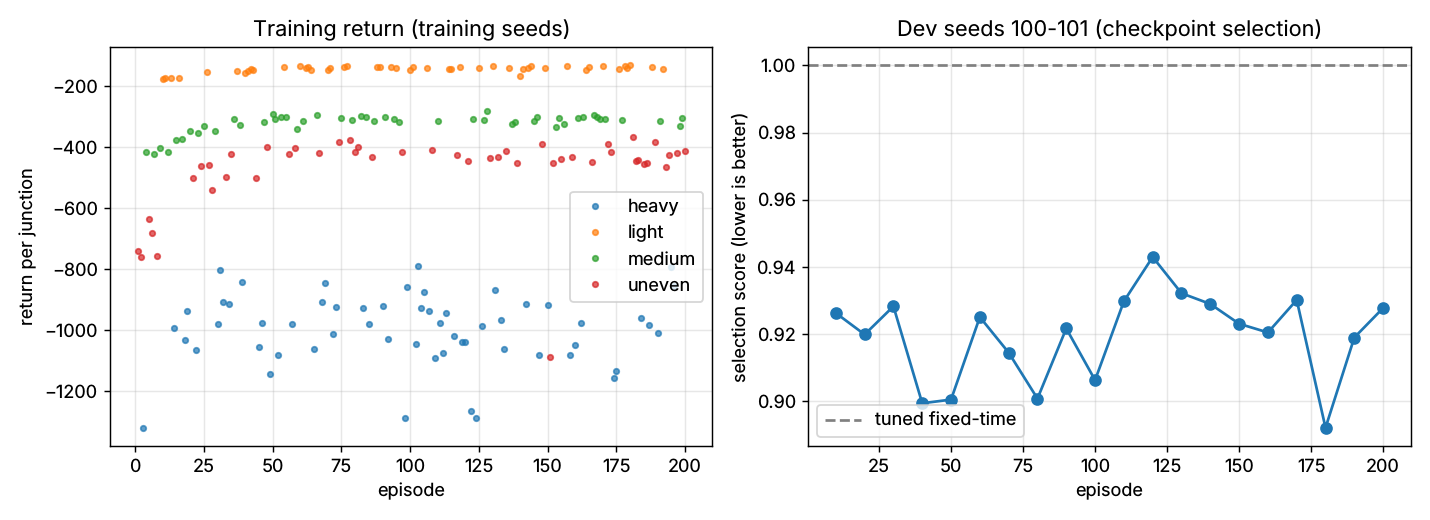
\includegraphics[width=\textwidth]{figures/results/dqn_training_curve.png}
\caption{DQN training return per junction and checkpoint-selection score on the development seeds}
\label{fig:dqn-training}
\end{figure}

\subsection{Ambulance Routing and Rerouting}

The routing graph in \path{manzil/routing/graph.py} uses SUMO edges as nodes. An arc joins two edges only when SUMO has a lane connection between them that an emergency vehicle may use, so every route can be driven and contains no U-turns. The edge cost follows Equation \ref{eq:edgecost}: the free-flow running time at the currently reported speed limit, plus 2 s per halting vehicle divided by the number of lanes, plus a declared 10 s signal delay on signalized edges, and an infinite cost for a closed edge. Snapshots older than five steps or with negative costs are rejected. Dijkstra is the reference search. A* uses the straight-line distance divided by the maximum speed, scaled by 0.896, the smallest ratio of edge length to node distance on the grid. The scaling is needed because SUMO edge lengths exclude the junction interiors, and it keeps the heuristic admissible.

The mission logic in \path{manzil/routing/mission.py} implements Algorithm \ref{alg:routing}. The route is refreshed every 5 s from the ambulance's current edge. A closure on the remaining route is accepted at once. Otherwise a cheaper route is adopted only if it saves more than $\delta=10$ s for at least $\tau=10$ s, with a 30 s cooldown after each revision. Each accepted route becomes a new numbered version with its trigger, and rejected candidates are logged. Static routing, used as the comparison arm, plans once on free-flow costs at dispatch.

\subsection{Green Corridor}

The corridor coordinator in \path{manzil/corridor/coordinator.py} implements Algorithm \ref{alg:corridor} with a look-ahead of the next two signalized junctions on the ambulance's remaining route. A junction is requested when it enters the look-ahead and activated when the ambulance's free-flow arrival time is within 15 s plus the time needed to clear the queue on its approach. Activation gives the corridor ownership of that junction in the safety filter, so normal requests are held, and the corridor requests the phase that serves the ambulance's movement. Priority lasts at most 60 s. Passage is detected when the ambulance leaves the approach edge, after which ownership returns to normal control through the safety filter, and recovery lasts until the junction's queue is back to its mean of the 120 s before activation. A route revision cancels requests at junctions that are no longer on the route.

A live dashboard run showed the ambulance stopping at red lights on its route, so the team added a per-second record of why the ambulance stood still and measured it in 20 runs per background controller. The main cause was a defect. After a route revision, SUMO keeps the edges already driven in the vehicle's route, so SUMO's route index was ahead of Manzil's route plan, and the corridor skipped the junction directly ahead of the ambulance. The coordinator now finds the ambulance's position by edge. With this fix the ambulance was never first in line at a red light at a corridor junction. Its remaining stops were vehicles queued in front of it and a permissive left turn at the final junction.

Four further changes were then tested on medium and heavy demand with five seeds and both fixed-time and DQN background control: earlier activation with a look-ahead of three junctions, shortening the current green for a corridor request, making ordinary vehicles give way with SUMO's blue-light device, and all three together. Only the shortened green was kept. In the resulting version of the corridor, a corridor request may end the current green after 5 s instead of the normal 10 s. Yellow and all-red are never shortened, normal control always keeps the full 10 s, and the safety monitor treats a green shorter than 10 s as a violation unless the corridor owns the junction, and a green shorter than 5 s as a violation in every case. Earlier activation gave small and inconsistent gains while increasing cross-street queueing by 4 to 14 percent. The blue-light device made the ambulance cross red lights; once red lights were enforced again, it caused gridlocks, because it needs SUMO's sublane model. It remains an option that is off by default. The measured effects are reported in Chapter \ref{ch:results}.

\subsection{Vehicle Detection, Tracking, and Counting}

Perception runs as three Kaggle jobs on two Tesla T4 GPUs. The first job, \path{kaggle/yolo_data}, builds the training data. UA-DETRAC labels four vehicle types, which are mapped to the project classes: car and van to car, bus to bus, and others to truck. Every tenth frame is used to avoid near-duplicates, regions that UA-DETRAC marks as ignored are filled grey, and the validation set consists of six whole training sequences, so frames of one sequence never appear in two splits. UA-DETRAC has no motorcycle labels, so COCO 2017 images that contain a motorcycle are added, with all four classes labelled, to stop the detector from forgetting that class. Table \ref{tab:vision-data} gives the resulting splits.

\begin{table}[htbp]
\centering
\caption{Detector training and test data}
\label{tab:vision-data}
\begin{tabularx}{\textwidth}{p{0.18\textwidth}YY}
\toprule
\textbf{Split} & \textbf{UA-DETRAC} & \textbf{COCO images with a motorcycle}\\
\midrule
Train & 7,365 frames from 54 sequences & 3,202 images\\
Validation & 867 frames from 6 whole sequences & 300 images\\
Test & 5,625 frames from the 40 official test sequences & --\\
Motorcycle test & -- & 159 images from COCO val2017\\
\bottomrule
\end{tabularx}
\end{table}

The second job, \path{kaggle/yolo_train}, fine-tunes the COCO-pretrained YOLO11s for 50 epochs at 640 pixels with batch size 32 and seed 0. Training took 1.8 h and the best validation epoch was 40. The 19 MB weights are kept in the repository with their SHA-256 checksum. The third job, \path{kaggle/yolo_track}, runs the fine-tuned detector with ByteTrack at the full 25 frames per second on all 40 test sequences, which is 56,340 frames, at 40 to 66 frames per second.

The counting logic in \path{manzil/perception/counting.py} is shared between the Kaggle job and the local tests. A full-width line is placed at 60 percent of the image height, and a track is counted once, when its box centre crosses the line, with its class taken as the majority over the track. Crossings inside ignored regions are dropped. Because UA-DETRAC gives true track identities, true counts are produced by passing the annotated boxes through the same counter, so the count error measures detection and tracking only. UA-DETRAC has no stop lines, so the queue indicator is a proxy: the number of tracked vehicles that moved less than a quarter of their box height in one second. A Kaggle script job must be a single file, so a build script copies the counting module into the job, and a test fails if that copy is out of date.

\subsection{Dashboard and API}

The FastAPI service in \path{manzil/api/} serves the built dashboard and the API on port 8000. One live run executes in a worker thread with the same step order as the batch runner: snapshot, routing, corridor, controller, safety filter, and adapter. Dashboard commands such as dispatching an ambulance or closing a road are queued and executed between two simulation steps, so only the worker thread touches SUMO. The live run uses the TraCI back end, so a SUMO failure cannot stop the API. The API offers run start, stop, and speed, network geometry, current state, ambulance dispatch, and road closure, and a WebSocket stream sends the state about ten times per second.

The dashboard in \path{dashboard/} is written in React 19 and TypeScript and built with Vite. It draws the network as plain SVG from the geometry in the SUMO network file. It shows the signal colour of every link at its stop line, the vehicles, queue shading on each road, closed roads, the ambulance with its current route version, and the corridor state of each junction. Chapter \ref{ch:manual} explains how to use it.

\subsection{Experiment Runner and Reproducibility}

The runner in \path{manzil/experiments/runner.py} validates a run configuration before starting SUMO and then executes Algorithm \ref{alg:loop}. Each run writes a folder with a manifest holding the configuration and its digest, the seed, the Manzil, SUMO, and Python versions, the Git commit, the network checksum, the demand record, the signal plan, the safety timing, and the termination reason. Next to the manifest are the metrics, a 60 s time series, the signal events, the applied controls, and, for emergency runs, the mission record with route versions, corridor events, and stop reasons. The batch tool runs controller arms, demand profiles, and seeds in parallel processes, and the comparison tool computes means, standard deviations, paired differences with 95 percent confidence intervals, and the number of seeds on which an arm was better. The comparison tool refuses to compare runs whose network, demand generator, protocol, or metric versions differ.

\section{Test Case Design and Description}

Manzil is a research prototype, so its tests serve two purposes: they check that each module behaves as specified, and they protect the experiments from software defects that would make a result meaningless. All tests are automated with pytest, and most of them start a real headless SUMO instance on the grid or a small scenario rather than replacing it with a mock. Table \ref{tab:test-suite} summarizes the suite. The tests share three conditions: the network is the committed 3$\times$3 grid unless stated otherwise, SUMO 1.28.0 is installed from the pinned package list, and runs are short (usually a few hundred simulated seconds) so that the suite finishes in a few minutes on the laptop.

\begin{longtable}{P{0.22\textwidth}P{0.07\textwidth}P{0.61\textwidth}}
\caption{Automated test suite}\label{tab:test-suite}\\
\toprule
\textbf{Test file} & \textbf{Tests} & \textbf{What is checked}\\
\midrule\endfirsthead
\caption[]{Automated test suite (continued)}\\
\toprule
\textbf{Test file} & \textbf{Tests} & \textbf{What is checked}\\
\midrule\endhead
\path{test_setup.py} & 5 & Package imports, SUMO installation, and tools\\
\path{test_grid.py} & 7 & Grid structure, checksum, and rebuild\\
\path{test_demand.py} & 12 & Seeded demand, rates, profile ordering, and no gridlock\\
\path{test_network.py} & 8 & Phases, conflict rule, and a second network\\
\path{test_adapter.py} & 5 & State reading, both back ends, and sole ownership of SUMO\\
\path{test_safety.py} & 13 & Transitions, minimum green, monitor, and maximum-red guard\\
\path{test_fixed_time.py} & 5 & Schedule windows and plan validation\\
\path{test_adaptive.py} & 9 & Equation \ref{eq:rule-score}, extension, maximum green, and hysteresis\\
\path{test_runner.py} & 12 & Run outputs, manifest, reproducibility, and configuration checks\\
\path{test_batch_compare.py} & 7 & Parallel batches, paired statistics, and incompatible runs\\
\path{test_routing.py} & 12 & Graph, costs, A* against Dijkstra, and rerouting rules\\
\path{test_emergency.py} & 6 & Ambulance missions, corridor lifecycle, closure, and timeout\\
\path{test_corridor_v2.py} & 7 & Route position, 5 s exception, red-light crossings, and stop reasons\\
\path{test_rl.py} & 7 & Observation layout, action mask, learning, and checkpoints\\
\path{test_counting.py} & 13 & Line counting, queue proxy, DETRAC parsing, and count errors\\
\path{test_yolo_data.py} & 6 & Class mapping, conversion, and sequence-level split\\
\path{test_api.py} & 13 & API validation, live run, dispatch, closure, reroute, and WebSocket\\
\midrule
\textbf{Total} & \textbf{147} & \\
\bottomrule
\end{longtable}

The test cases below describe the most important behaviours in the format used for the project: each case states its objective, the requirement it verifies, the preconditions, the steps, and the expected and actual results. Every case corresponds to one or more automated tests, named in the last row, so the result can be reproduced by running those tests.

\begin{table}[htbp]
\centering
\caption{TC-01: Invalid run configurations are rejected}
\label{tab:tc01}
\begin{tabularx}{\textwidth}{p{0.22\textwidth}Y}
\toprule
\textbf{Field} & \textbf{Description}\\
\midrule
Objective & Verify that a run with a missing or invalid setting never starts.\\
Requirement & FR-01\\
Module & Experiment runner and API\\
Precondition & SUMO installed; no run active.\\
Steps & 1. Submit six run configurations, each with one invalid field: an unknown profile, controller, or scenario, a negative seed, a zero measurement length, or a fractional warm-up.\newline 2. Submit five invalid start requests to the API (unknown controller or profile, negative seed or speed, too short a duration).\\
Expected result & Each configuration is refused with an ``invalid run config'' error and no manifest is written; the API answers with HTTP 422 and stays idle.\\
Actual result & As expected for all eleven inputs.\\
Status & Passed\\
Automated tests & \path{test_runner.py::test_bad_config_rejected_before_start}, \path{test_api.py::test_bad_start_requests_are_rejected}\\
\bottomrule
\end{tabularx}
\end{table}

\begin{table}[htbp]
\centering
\caption{TC-02: The adapter is the sole owner of SUMO}
\label{tab:tc02}
\begin{tabularx}{\textwidth}{p{0.22\textwidth}Y}
\toprule
\textbf{Field} & \textbf{Description}\\
\midrule
Objective & Verify that no module other than the adapter can step SUMO or change a signal.\\
Requirement & FR-03\\
Module & Simulation adapter\\
Precondition & Source code of the \texttt{manzil} package.\\
Steps & 1. Scan every Python file in the package for an import of \texttt{traci} or \texttt{libsumo}.\newline 2. Run the grid with both back ends and compare the lane states.\\
Expected result & Only \path{adapter.py} imports SUMO, and both back ends report identical states.\\
Actual result & No other module imports SUMO; states are identical.\\
Status & Passed\\
Automated tests & \path{test_adapter.py::test_adapter_is_sole_owner_of_sumo}, \path{test_adapter.py::test_both_backends_agree}\\
\bottomrule
\end{tabularx}
\end{table}

\begin{table}[htbp]
\centering
\caption{TC-03: Signal changes follow the legal transition}
\label{tab:tc03}
\begin{tabularx}{\textwidth}{p{0.22\textwidth}Y}
\toprule
\textbf{Field} & \textbf{Description}\\
\midrule
Objective & Verify that a requested phase change passes through minimum green, yellow, and all-red, and that it is recorded.\\
Requirement & FR-07, FR-08\\
Module & Safety filter\\
Precondition & Safety filter reset on the grid; current phase green since time 0.\\
Steps & 1. Request phase 1 after 5 s of green.\newline 2. Request phase 1 after 10 s of green.\newline 3. Read the shown signal state for each second from 10 s to 16 s.\\
Expected result & The first request is held (minimum-green hold) and phase 0 stays green; the second is applied with 3 s of yellow, 2 s of all-red, and the new green at 15 s, and is stored as an applied-control record.\\
Actual result & As expected.\\
Status & Passed\\
Automated tests & \path{test_safety.py::test_switch_held_until_min_green}, \path{test_safety.py::test_full_switch_sequence}\\
\bottomrule
\end{tabularx}
\end{table}

\begin{table}[htbp]
\centering
\caption{TC-04: A random controller cannot produce an unsafe signal}
\label{tab:tc04}
\begin{tabularx}{\textwidth}{p{0.22\textwidth}Y}
\toprule
\textbf{Field} & \textbf{Description}\\
\midrule
Objective & Verify that the safety filter keeps every shown state legal whatever a controller requests.\\
Requirement & FR-08\\
Module & Safety filter and safety monitor\\
Precondition & Light demand on the grid.\\
Steps & 1. Let a controller request random phases at random times for 5,000 steps without SUMO.\newline 2. Repeat for 600 steps in real SUMO, with the monitor reading the states SUMO reports.\\
Expected result & No conflicting greens, no green without a preceding yellow, no short yellow or green; more than 50 yellow intervals occur, so the filter is actually exercised.\\
Actual result & Zero violations in both runs.\\
Status & Passed\\
Automated tests & \path{test_safety.py::test_random_requests_never_unsafe_without_sumo}, \path{test_safety.py::test_random_requests_never_unsafe_in_sumo}\\
\bottomrule
\end{tabularx}
\end{table}

\begin{table}[htbp]
\centering
\caption{TC-05: The maximum-red guard serves a starved phase}
\label{tab:tc05}
\begin{tabularx}{\textwidth}{p{0.22\textwidth}Y}
\toprule
\textbf{Field} & \textbf{Description}\\
\midrule
Objective & Verify that the safety layer, not the controller, has the last word on maximum red, and that it does not override an active corridor.\\
Requirement & FR-08; NFR on fairness\\
Module & Safety filter\\
Precondition & Maximum red set to 40 s for the test.\\
Steps & 1. Let a controller request phase 0 for 200 s.\newline 2. Repeat while the corridor owns the junction.\\
Expected result & The filter forces phase 1 at 35 s (40 s minus 5 s clearance) and no phase waits longer than 45 s; under corridor ownership the guard does not act.\\
Actual result & As expected; zero monitor violations.\\
Status & Passed\\
Automated tests & \path{test_safety.py::test_max_red_guard_forces_service}, \path{test_safety.py::test_max_red_guard_does_not_override_the_corridor}\\
\bottomrule
\end{tabularx}
\end{table}

\begin{table}[htbp]
\centering
\caption{TC-06: A* returns optimal routes}
\label{tab:tc06}
\begin{tabularx}{\textwidth}{p{0.22\textwidth}Y}
\toprule
\textbf{Field} & \textbf{Description}\\
\midrule
Objective & Verify that A* with the scaled heuristic finds the same cost as Dijkstra and never expands more nodes.\\
Requirement & FR-10\\
Module & Routing graph\\
Precondition & Routing graph built from the grid.\\
Steps & 1. Draw 200 random cost sets and random origin and destination edges.\newline 2. Solve each with Dijkstra and with A*.\newline 3. Check the heuristic against the true cost for all 48$\times$48 edge pairs.\\
Expected result & Equal path costs, A* expands no more nodes, and the heuristic never exceeds the true cost.\\
Actual result & As expected for all 200 cases and all pairs.\\
Status & Passed\\
Automated tests & \path{test_routing.py::test_astar_matches_dijkstra_on_random_costs}, \path{test_routing.py::test_heuristic_is_admissible}\\
\bottomrule
\end{tabularx}
\end{table}

\begin{table}[htbp]
\centering
\caption{TC-07: Invalid ambulance missions are reported}
\label{tab:tc07}
\begin{tabularx}{\textwidth}{p{0.22\textwidth}Y}
\toprule
\textbf{Field} & \textbf{Description}\\
\midrule
Objective & Verify that an invalid origin or destination is refused and that a disconnected destination is reported.\\
Requirement & FR-09\\
Module & Routing mission and API\\
Precondition & Routing graph built from the grid.\\
Steps & 1. Dispatch from a road that does not exist.\newline 2. Dispatch a valid mission, then close every road into the destination.\newline 3. Send dispatches to the API with an unknown origin and with the same origin and destination.\\
Expected result & Step 1 is refused; step 2 sets the mission to NO\_ROUTE; both requests in step 3 are refused with HTTP 409.\\
Actual result & As expected.\\
Status & Passed\\
Automated tests & \path{test_routing.py::test_dispatch_rejects_bad_endpoints}, \path{test_routing.py::test_no_route_reported}, \path{test_api.py::test_bad_dispatch_is_rejected}\\
\bottomrule
\end{tabularx}
\end{table}

\begin{table}[htbp]
\centering
\caption{TC-08: A road closure triggers a new route and cancels obsolete priority}
\label{tab:tc08}
\begin{tabularx}{\textwidth}{p{0.22\textwidth}Y}
\toprule
\textbf{Field} & \textbf{Description}\\
\midrule
Objective & Verify that closing a road on the ambulance's route produces a new route version, that the ambulance avoids the road, and that corridor requests on the old route are cancelled.\\
Requirement & FR-11, FR-14\\
Module & Routing mission and corridor coordinator\\
Precondition & Medium demand; ambulance dispatched with the corridor on.\\
Steps & 1. Run the mission once without a closure to obtain route 1.\newline 2. Repeat with the same seed and close the fourth road of route 1 shortly after dispatch.\\
Expected result & The mission arrives; the first revision has trigger ``closure''; the closed road is not driven; route versions are numbered 1, 2, \ldots; a corridor request is cancelled with reason route\_v2; no safety violation or teleport.\\
Actual result & As expected.\\
Status & Passed\\
Automated tests & \path{test_emergency.py::test_closure_triggers_new_route_version_and_cancels_priority}\\
\bottomrule
\end{tabularx}
\end{table}

\begin{table}[htbp]
\centering
\caption{TC-09: The corridor follows its lifecycle and releases safely}
\label{tab:tc09}
\begin{tabularx}{\textwidth}{p{0.22\textwidth}Y}
\toprule
\textbf{Field} & \textbf{Description}\\
\midrule
Objective & Verify that each corridor junction passes through the states of Algorithm \ref{alg:corridor} in order and returns to normal control, also when priority times out.\\
Requirement & FR-12, FR-13\\
Module & Corridor coordinator\\
Precondition & Ambulance mission with the corridor on.\\
Steps & 1. Run a mission and collect the corridor events of every junction.\newline 2. Repeat with a maximum priority of only 2 s to force timeouts.\\
Expected result & States appear in the order REQUESTED, SAFE TRANSITION, ACTIVE PRIORITY, PASSAGE, RECOVERY, IDLE; normal requests are held while the corridor owns a junction; after a timeout the ambulance still arrives and no violation occurs.\\
Actual result & As expected.\\
Status & Passed\\
Automated tests & \path{test_emergency.py::test_corridor_lifecycle_order_and_safety}, \path{test_emergency.py::test_priority_timeout_releases_safely}\\
\bottomrule
\end{tabularx}
\end{table}

\begin{table}[htbp]
\centering
\caption{TC-10: The 5 s corridor minimum applies only to the corridor}
\label{tab:tc10}
\begin{tabularx}{\textwidth}{p{0.22\textwidth}Y}
\toprule
\textbf{Field} & \textbf{Description}\\
\midrule
Objective & Verify that only a corridor request may end a green after 5 s, that clearance is never shortened, and that the ambulance never crosses a red light.\\
Requirement & FR-08\\
Module & Safety filter, safety monitor, and ambulance driver\\
Precondition & Corridor minimum green set to 5 s.\\
Steps & 1. Submit a normal request after 6 s of green.\newline 2. Submit corridor requests after 4 s and after 6 s of green.\newline 3. Show the monitor a 6 s green under normal ownership and a 4 s green under corridor ownership.\newline 4. Run an ambulance mission without the corridor and record the signal at every stop line it crosses.\\
Expected result & The normal request and the 4 s corridor request are held; the 6 s corridor request switches with 3 s yellow and 2 s all-red; the monitor flags both short greens; the ambulance crosses at least four stop lines and none on red.\\
Actual result & As expected.\\
Status & Passed\\
Automated tests & \path{test_corridor_v2.py::test_truncation_only_for_the_corridor_and_never_clearance}, \path{test_corridor_v2.py::test_monitor_flags_truncation_without_corridor_ownership}, \path{test_corridor_v2.py::test_plain_ambulance_never_crosses_on_red}\\
\bottomrule
\end{tabularx}
\end{table}

\begin{table}[htbp]
\centering
\caption{TC-11: Runs are reproducible and incompatible runs are not compared}
\label{tab:tc11}
\begin{tabularx}{\textwidth}{p{0.22\textwidth}Y}
\toprule
\textbf{Field} & \textbf{Description}\\
\midrule
Objective & Verify that the same configuration gives the same metrics and that the comparison tool refuses runs with different settings.\\
Requirement & FR-17, FR-18\\
Module & Experiment runner, batch, and comparison tools\\
Precondition & Short medium-demand runs.\\
Steps & 1. Run the same configuration twice, and once more with the TraCI back end.\newline 2. Run a batch in parallel and the same run serially.\newline 3. Change the measurement length of one row and request a comparison.\\
Expected result & Identical metrics in steps 1 and 2; the manifest records every reproducing setting; step 3 is refused as incompatible.\\
Actual result & As expected.\\
Status & Passed\\
Automated tests & \path{test_runner.py::test_same_seed_same_metrics}, \path{test_runner.py::test_traci_backend_gives_the_same_metrics}, \path{test_batch_compare.py::test_parallel_batch_matches_a_serial_run}, \path{test_batch_compare.py::test_incompatible_runs_refused}\\
\bottomrule
\end{tabularx}
\end{table}

\begin{table}[htbp]
\centering
\caption{TC-12: Vehicles are counted once at the counting line}
\label{tab:tc12}
\begin{tabularx}{\textwidth}{p{0.22\textwidth}Y}
\toprule
\textbf{Field} & \textbf{Description}\\
\midrule
Objective & Verify the counting rule used for the count-error results.\\
Requirement & FR-04, FR-05\\
Module & Perception counting\\
Precondition & Counting line defined on a synthetic frame sequence.\\
Steps & 1. Move a tracked box down across the line with jitter back over it.\newline 2. Move a box back and forth across the line inside an ignored region.\newline 3. Track stopped and moving boxes for the queue proxy.\\
Expected result & Step 1 gives exactly one ``down'' event at the first crossing; step 2 gives no event; only stopped vehicles count towards the queue.\\
Actual result & As expected.\\
Status & Passed\\
Automated tests & \path{test_counting.py::test_vehicle_moving_down_is_counted_once}, \path{test_counting.py::test_crossing_in_ignored_region_dropped_and_not_recounted}, \path{test_counting.py::test_queue_estimator_stopped_vs_moving}\\
\bottomrule
\end{tabularx}
\end{table}

\begin{table}[htbp]
\centering
\caption{TC-13: Dashboard session from dispatch to rerouting}
\label{tab:tc13}
\begin{tabularx}{\textwidth}{p{0.22\textwidth}Y}
\toprule
\textbf{Field} & \textbf{Description}\\
\midrule
Objective & Verify the operator workflow through the API used by the dashboard.\\
Requirement & FR-02, FR-15\\
Module & FastAPI service and live session\\
Precondition & API started; no run active.\\
Steps & 1. Start a medium-demand run and slow it to three times real time.\newline 2. Dispatch an ambulance from left0A0 to C2top2 with the corridor on; send a second dispatch.\newline 3. Close the fourth road of the route; close it again; close a road that does not exist.\newline 4. Wait for a new route version.\\
Expected result & The first dispatch is accepted and the second refused (one mission at a time); the first closure is accepted and the repeated and unknown closures refused; route version 2 avoids the closed road.\\
Actual result & As expected.\\
Status & Passed\\
Automated tests & \path{test_api.py::test_dispatch_close_road_reroute_and_corridor}\\
\bottomrule
\end{tabularx}
\end{table}

\section{Test Metrics}

Table \ref{tab:test-metrics} summarizes the result of the last full test run on the team laptop, and Table \ref{tab:traceability} links each functional requirement of Table \ref{tab:functional-requirements} to its implementation status at the end of FYP-I and to the test cases that verify it. A requirement is marked implemented only when code and passing tests exist; partial and planned requirements name the missing part, which is carried into the FYP-II plan in Chapter \ref{ch:conclusion}.

\begin{table}[htbp]
\centering
\caption{Test metrics}
\label{tab:test-metrics}
\begin{tabularx}{\textwidth}{Yp{0.30\textwidth}}
\toprule
\textbf{Metric} & \textbf{Value}\\
\midrule
Automated tests & 147 in 17 files\\
Tests passed & 147\\
Tests failed or skipped & 0\\
Documented test cases (TC-01 to TC-13) & 13, all passed\\
Functional requirements covered by a documented test case & 17 of 20\\
Safety violations in all reported experiment runs & 0\\
\bottomrule
\end{tabularx}
\end{table}

\begin{longtable}{P{0.08\textwidth}P{0.36\textwidth}P{0.30\textwidth}P{0.14\textwidth}}
\caption{Requirement traceability and FYP-I status}\label{tab:traceability}\\
\toprule
\textbf{ID} & \textbf{Requirement (short)} & \textbf{Status} & \textbf{Test cases}\\
\midrule\endfirsthead
\caption[]{Requirement traceability and FYP-I status (continued)}\\
\toprule
\textbf{ID} & \textbf{Requirement (short)} & \textbf{Status} & \textbf{Test cases}\\
\midrule\endhead
FR-01 & Validate scenario configuration & Implemented & TC-01\\
FR-02 & Start, pause, resume, stop a run & Partial: start, stop, and speed; no pause & TC-13\\
FR-03 & Adapter is sole owner of SUMO & Implemented & TC-02\\
FR-04 & Process recorded video & Partial: offline batch job on Kaggle & TC-12\\
FR-05 & Aggregate observations & Partial: per-sequence counts and per-frame queue proxy & TC-12\\
FR-06 & Select the controller & Implemented & TC-13\\
FR-07 & Record every signal action & Implemented & TC-03\\
FR-08 & Minimum green and clearance & Implemented; 5 s minimum for corridor requests & TC-03, TC-04, TC-05, TC-10\\
FR-09 & Validate ambulance endpoints & Implemented & TC-07\\
FR-10 & Time-based route & Implemented & TC-06\\
FR-11 & Reroute on closure or improvement & Implemented & TC-08\\
FR-12 & Bounded corridor look-ahead & Implemented & TC-09\\
FR-13 & Passage, cancellation, recovery & Implemented & TC-09\\
FR-14 & Cancel obsolete priority & Implemented & TC-08\\
FR-15 & Dashboard state display & Partial: simulation source only & TC-13\\
FR-16 & Visible stale and fallback states & Planned for FYP-II & --\\
FR-17 & Record configuration and events & Implemented & TC-11\\
FR-18 & Compatible comparisons only & Implemented & TC-11\\
FR-19 & Export run data & Partial: JSON and CSV run files; no export command & --\\
FR-20 & Fallback for the learned controller & Partial: holds the current legal phase & --\\
\bottomrule
\end{longtable}

Thirteen requirements are implemented, six are partial, and one is planned. FR-08 is met for every normal controller; the only exception is the shortened 5 s minimum for corridor requests described in the corridor section, which the safety monitor checks in every run. For FR-20 the implemented fallback keeps the current legal phase and counts the event instead of switching to fixed-time control. This is simpler but still safe, because the safety filter controls every transition.

\section{Conclusion}

The FYP-I implementation turns the design of Chapter \ref{ch:design} into a working prototype: a reproducible SUMO grid with seeded demand, a single simulation adapter, a safety filter that every controller must pass through, three signal controllers including a trained DQN, time-based routing with closure-triggered rerouting, a moving green corridor, a fine-tuned detection, tracking, and counting pipeline, and a live dashboard. The implementation also uncovered problems that a demonstration alone would have hidden, namely a misleading travel-time metric, a starvation case that led to the maximum-red guard, and the corridor's route-index defect, and each was fixed and covered by a test. All 147 automated tests pass. Chapter \ref{ch:manual} explains how to operate the prototype, and Chapter \ref{ch:results} reports the experiments run with it.
